\section{Umsetzung}
\label{sec:software}
Nachdem nun die Grundlagen und das prinzipielle Vorgehen zur Lösung klar sind, folgt hier eine kurze Darstellung der entwickelten Software. Zusätzlich findet sich eine ausführliche Dokumentation als Kommentare im Quelltext sowie in den Java-Doc-Pages. Bei Detailfragen sei darauf verwiesen. \par

\subsection{Wesentlichen Eigenschaften}
Folgende Richtlinien wurden bei dem Design und der Entwicklung der Software beachtet:

\begin{description}
\item[fail-early]
Die Software soll so entwickelt werden, dass die Parameter der Methoden unmittelbar auf ihren Gültigkeitsbereich überprüft werden, so dass Fehler frühzeitig erkannt und auch dem Nutzer mitgeteilt werden können. 

\item[report-early]
Die Software soll so entwickelt werden, dass sie den Nutzer möglichst gut Auskunft darüber gibt bzw. geben kann, was sie gerade tut. 

\item[Bezeichner]
Die Software soll so entwickelt werden, dass die verwendeten Bezeichner für Variablen, Methoden, Klassen und Paketen einheitlich und unmittelbar einsichtig sind, und Auskunft über die Funktion bzw. Bedeutung geben. Um lange Bezeichner zu vermeiden, werden eingängige und einheitliche Abkürzungen verwendet.\par

\item[Mehr Kommentare sind besser als weniger]
Die Software soll möglichst umfangreich und mit Hilfe von Java-Doc-Tags kommentiert werden. Das heißt, Klassen und Methoden, die sich nicht unmittelbar selbst erklären, sollen eine Beschreibung ihrer Funktion, Parameter und Besonderheiten enthalten. Zudem soll auch die interne Struktur und Funktionsweise mit Hilfe von Kommentaren begleitend erläutert werden.

\item[Frühes Abstrahieren und Kapselung]
Das Design der Software soll so geschehen, dass ein möglichst hoher Grad an Abstraktion und Kapselung erreicht wird. Das macht die Software leichter verständlich und nutzbar, erweiterbarer, wiederverwendbarer und weniger fehleranfällig.

\item[Sprache]
Die Sprache des Quellcodes und der Kommentare im Quellcode ist Englisch.
\end{description}

Dem Design lagen folgende Entscheidungen zugrunde:
\begin{description}
\item[Programmiersprache]
Da der Großteil des Semedico Projekts in Java entwickelt wurde, fiel die Wahl auch für diese Studienarbeit automatisch auf Java. \par

%Zwar interagiert die entwickelte Software im Moment nicht direkt mit Semedico, allerdings ist so gewährleistet, dass ggf. eine Integration problemlos möglich ist.

\item[Entwicklungsumgebung]
Als Entwicklungsumgebung wird Eclipse verwendet. Dies geschieht aus zwei Gründen: Erstens habe ich bereits Erfahrungen mit Eclipse und zweitens wird auch zur Entwicklung von Semedico Eclipse verwendet. 

\item[Versionsmanagement]
Da für das Semedico Projekt bereits ein SVN-Repository existiert, wurde diese, inklusive des Maven-Build-Managements, übernommen.

\item[XML-Parser]
Die XML-Daten des MeSH haben eine ungefähre Größe von 300\,MB. Daher ist es eminent wichtig einen XML-Parser zu verwenden, der erstens mit Dateien dieser Größe umgehen kann und zweitens diese auch in kurzer Zeit verarbeiten kann. \par 

Der klassische XML-Parser JDOM hat sich bei einem kurzem Test als vollkommen unbrauchbar herausgestellt. JDOM muss jederzeit ein komplettes Abbild der XML-Daten im Speicher halten und wird damit bei diesen Datenmengen extrem langsam bzw. stürzt ab. \par

Die Wahl fiel daher auf die Simple API for XML (SAX) in Form des Java-SAX-Parser, der über die Pakete \code{org.xml.sax.*} zur Verfügung gestellt wird. Dieser arbeitet sequentiell und push-event-basiert. Dadurch ist SAX deutlich schneller und minimiert den Speicherbedarf. \par

Eine mögliche Alternative ist die Streaming API for XML (StAX). Jedoch erscheint die strikt sequentielle Verarbeitungsweise von SAX hier passender und für diese Anwendung effizienter und leichter umsetzbar.

\item[Graphenbibliothek]
Als Graphenbibliothek wird die etablierte JGraphT-Bibliothek verwendet. 
\end{description}

\subsection{Design}

\begin{figure}[h]
\begin{center}
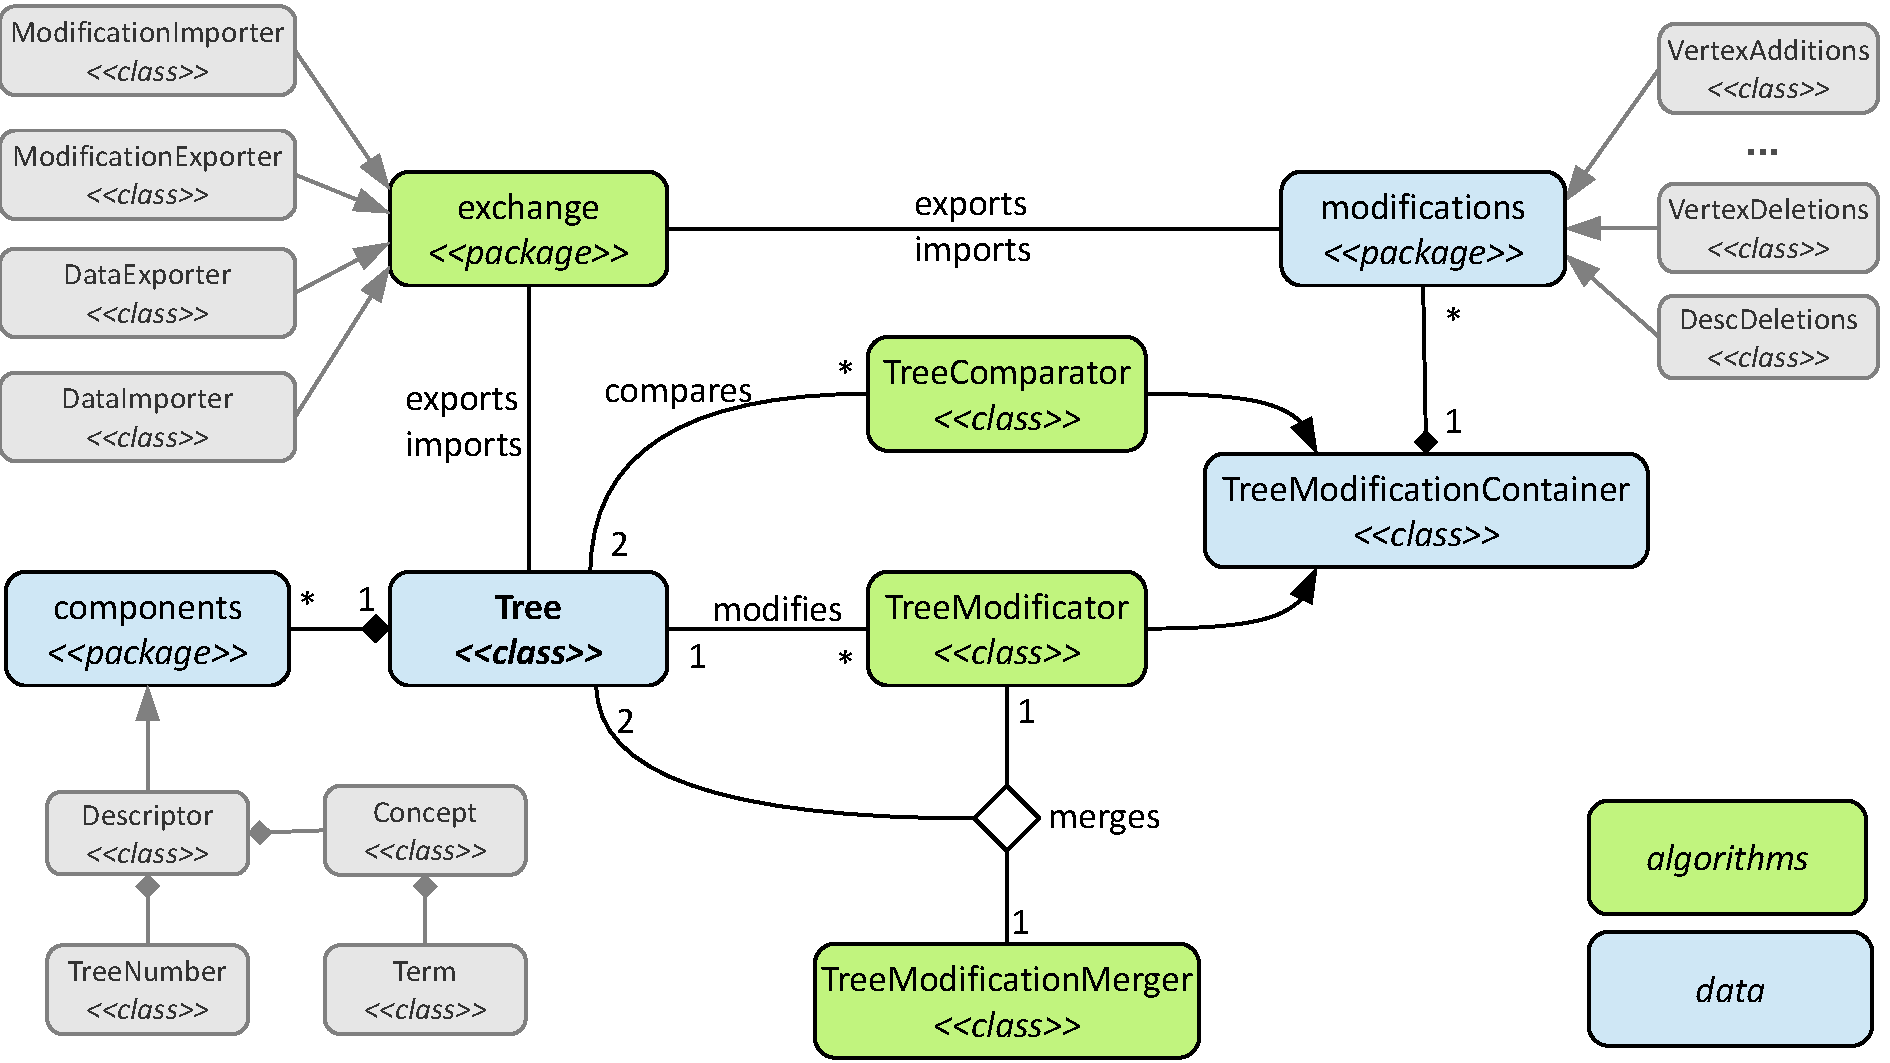
\includegraphics[width=1.0\textwidth]{figs/sw_overview3.pdf}
\end{center}
\caption{Überblick zur Struktur der Software}
\label{figs:sw_overview}
\end{figure}

\autoref{figs:sw_overview} zeigt einen Überblick zur Struktur und dem Zusammenspiel der wichtigsten Klassen und Packages. Die Darstellung ist an UML-Klassen-Diagramme angelehnt. \par

Im Zentrum steht die \code{Tree}-Klasse. Sie repräsentiert einen MeSH-Tree. \par

Der Import und Export von Modifikationen und Daten für \code{Tree} wird von Klassen im \code{exchange}-Package übernommen. \par

Unterschiede zwischen zwei MeSH-Trees können über eine Instanz der Klasse \code{TreeComparator} bestimmt werden. Diese implementieren die Algorithmen aus \ref{sec:vergleichBaume} \nameref{sec:vergleichBaume}. \par

Eine Aktualisierung von Modifikationen, wie in \ref{sec:merging} \nameref{sec:merging} beschrieben, kann durch eine Instanz der Klasse \code{TreeModificationMerger} berechnet werden.\par

Instanzen der Klasse \code{TreeModificator} erlauben es Instanzen von \code{Tree} zu verändern.\par

\code{TreeComparator} und \code{TreeModificator} leiten von der selben Basisklasse \code{TreeModificationContainer} ab, da beide ein Menge von Modifikationen verwalten. Deshalb kann das Ergebnis eines Vergleichs zweier Bäume, also ein \code{TreeComparator}-Objekt, leicht in eine Instanz von \code{TreeModificator} überführt werden, und umgekehrt. \par

Die möglichen Modifikationen entsprechen den in \ref{sec:mesh_operationen} \nameref{sec:mesh_operationen} aufgelisteten Operationen.

\subsection{Package-Übersicht}
Die Software ist in eine Reihe von Packages aufgeteilt, die jeweils für sich eine funktionale Einheit bilden. Eine Übersicht bietet \autoref{table:package_übersicht}. \par

\begin{table}[h]
\begin{center}
\begin{tabularx}{0.8\textwidth}{rX}
\toprule
\textbf{Package-Name} & \textbf{Erläuterung} \\ \midrule
Basis-Package & Enthält alle andere Pakete sowie die wesentlichen Klassen der Software. Dazu gehören insbesondere die Klassen \code{Process}, \code{Tree}, \code{TreeComparator}, \code{TreeModificator} und \code{TreeModificationMerger}. \\ \midrule
\code{components} & Beschreibt die wesentlichen MeSH-XML-Elemente, wie \code{Descriptor}, \code{Concept} oder \code{Term}, als einzelne Klassen. \\ \midrule
\code{exchange} & Für Import bzw. Export der MeSH-Daten und Modifikationen. Verschiedene Formate werden unterstützt. \\ \midrule
\code{modifications} & Beschreibt Modifikationen die auf MeSH-Trees angewandt werden können, wie \code{DescAdditions} oder \code{VertexDeletions}. \\ \midrule 
\code{testing} & JUnit-Testing-Klassen. \\ \midrule   
\code{tools} & Verschiedene Hilfsklassen und Methoden. \\ \bottomrule 
\end{tabularx}
\end{center}
\caption{Package-Übersicht}
\label{table:package_übersicht}
\end{table}

\subsection{Klassen-Übersicht}
In \autoref{table:class_übersicht} sind die wichtigsten Klassen zusammen mit ihrer Funktion aufgeführt.

\begin{table}
\begin{center}
\begin{tabularx}{1.05\textwidth}{rX}
\toprule
\textbf{Klassenname} & \textbf{Erläuterung} \\ \midrule
% \textit{Basis-Package} & \\ \midrule
%\multicolumn{2}{l}{\textit{Basis-Package}} \\ \midrule
\code{Process} & Beispielanwendung, welche die entwickelte Bibliothek nutzt. \\ \midrule

\code{Tree} & Repräsentation eines MeSH-Trees. \code{Tree} stellt elementare Methoden zum Modifizieren und Abfragen eines MeSH-Trees zur Verfügung. Dies umfasst beispielsweise Tree-Vertices löschen, verschieben oder hinzufügen. \\ \midrule
% Objekte dieser Klasse können über Methoden in \code{exchange} aus Daten unterschiedlichen Formats importiert sowie in verschiedene Formate exportiert werden. 

\code{TreeComparator} & Abstrakte Basisklasse um zwei MeSH-Trees zu vergleichen. Bestimmt dabei die Modifikationen, die den einen MeSH-Tree in den anderen überführen. \\ \midrule

\code{TreeComparatorMeSH} &  Ableitung der Klasse \code{TreeComparator}. Vergleicht zwei beliebige \code{Tree}-Instanzen. Implementiert die Methoden aus \ref{sec:vergleichBaume} \nameref{sec:vergleichBaume}. \\ \midrule

\code{TreeComparatorUD} & Ableitung der Klasse \code{TreeComparator}. Vergleich eine beliebige \code{Tree}-Instanz mit einer \code{Tree}-Instanz zu vergleichen, welche aus UD-XML-Daten (siehe \autoref{sec:sw_details}) erstellt wurde. \\ \midrule

\code{TreeFilter} & Zum Filtern von unerwünschten Tree Vertices oder Descriptors aus einem \code{Tree}-Objekt. Existiert unabhängig von den anderen Klassen zum Modifizieren.\\ \midrule

\code{TreeModificationContainer} &  Container für Tree-Modifikationen. Basisklasse für \code{TreeModificator} und \code{TreeComparator}. \\ \midrule

\code{TreeModificationMerger} & Zum Aktualisieren einer Instanz von \code{TreeModificationContainer} für ein verändertes \code{Tree}-Objekt. Implementierung der Methoden aus \ref{sec:merging} \nameref{sec:merging}.  \\ \midrule

\code{TreeModificator} &  Ableitung der Klasse \code{TreeModificationContainer}. Ermöglicht die Anwendung der enthaltenen Modifikationen auf ein \code{Tree}-Objekt. \\ \midrule

% \textit{\code{components}-Package} & \\ \midrule
% \code{Concept} & Repräsentation eines MeSH-Concepts. \\ \midrule
% \code{Descriptor} & Repräsentation eines MeSH-Descriptors. \\ \midrule
% \code{Term} &  Repräsentation eines MeSH-Terms.\\ \midrule
%\code{TreeNumber} &  Repräsentation einer MeSH-TreeNumber beim Import von MeSH-XML-Daten. Wird in \code{TreeVertex} überführt. Siehe dazu auch \ref{sec:repräsentation_des_mesh_als_baum} \nameref{sec:repräsentation_des_mesh_als_baum}. \\ \midrule
%\code{TreeVertex} & Interne Repräsentation einer MeSH-TreeNumber. \\ \midrule

%\toprule
%\textit{\code{ }-Package} & \\ \midrule
\code{DataExporter} &  Exportieren eines \code{Tree}-Objekts in verschiedene Formate. Neben dem Own-XML-Format (siehe \autoref{sec:sw_details}), wird auch ein direktes Exportieren in das Semedico-Datenbankmanagementsystem (DBMS) unterstützt. \\ \midrule
%\code{DataImporter} &  Importieren verschiedener Formate für \code{Tree}-n ein \code{Tree}-Objects in verschiedene Formate. \\ \midrule
\code{Parser4MeSH} & SAX-XML-Handler um MeSH-XML-Dokumente zu parsen. \\ \midrule
\code{Parser4OwnMeSH} & SAX-XML-Handler um Dokumente mit einer MeSH-XML-ähnlichen Syntax zu parsen. Siehe auch \autoref{sec:sw_details}. \\ \midrule
\code{Parser4UserDefMeSH} & SAX-XML-Handler um XML-Dokumente zu parsen, die mit dem alten Algorithmus zum Erstellen des Semedico-MeSH erzeugt wurden. \\ \bottomrule
\end{tabularx}
\end{center}
\caption{Klassen-Übersicht}
\label{table:class_übersicht}
\end{table}

\subsection{Interessante Details}
\label{sec:sw_details}
\minisec{XML-Formate}
Es werden im Moment drei XML-Formate unterstützt:

\begin{description}
\item[UD-XML] Der bisher zu Erstellung des Semedico-MeSH verwandte Algorithmus speichert seine Ergebnisse in einem eigenen XML-Format. Dieses Format wird hier als UD-XML bezeichnet. Die Klasse \code{Parser4UserDefMeSH} implementiert einen SAX-XML-Handler zum Einlesen. Ein Schreiben ist nicht möglich.

\item[MeSH-XML] Dies ist das offizielle und bereits in \ref{sec:xml_struktur} \nameref{sec:xml_struktur} beschrieben XML-Format des MeSH. Die Klasse \code{Parser4MeSH} implementiert den entsprechenden SAX-XML-Handler zum Einlesen. Ein Schreiben ist nicht möglich. Stattdessen kann dazu das Own-XML-Format verwendet werden. 

\item[Own-XML] Eigenes XML-Format, das eine leicht veränderte Teilmenge des MeSH-XML-Formats darstellt: \par

Nur die XML-Elemente, welche auch in \code{Tree}-Objekten repräsentiert werden, wurden übernommen. \par

Statt des XML-Elements \code{<TreeNumberList>} samt \code{<TreeNumber>}s, gibt es nun ein XML-Element \code{<LocationList>} mit den Kindern \code{<Location>}, welche selbst aus \code{<ParentVertexName>} und \code{<VertexName>} bestehen. Der Sinn ist es, die Struktur des MeSH explizit als Relation festzuhalten. Siehe dazu auch in \ref{sec:xml_struktur} den Unterpunkt Tree Number. \par
 
Die Klasse \code{Parser4OwnMesh} implementiert einen SAX-XML-Handler zum Einlesen. Schreiben ist über zwei überladene Methoden \code{toOwnXml} der Klasse \code{DataExporter} möglich.
\end{description}

\minisec{Descriptor-Additionen in \code{Tree}-Objekte}
Da die MeSH-XML-Daten als Menge von Descriptors organisiert sind, geschieht auch das Einlesen der XML-Daten als Iteration über alle \code{<DescriptorRecord>}-Elemente. Und weil Descriptors jeweils eine Menge aus Tree Vertices besitzen, und diese an beliebigen Stellen im Tree-Vertex-Baum verteilt sein können, sind wir mit einem Problem konfrontiert: Es müssen ggf. Tree-Vertices eingefügt werden, deren Väter noch nicht im MeSH-Tree existieren. \par 

Um diese Problem zu lösen, verwaltet jedes \code{Tree}-Objekt eine \code{pendingVertices}-Map: Schlüssel der Map sind die noch fehlenden Vater-Tree-Vertices. Die Werte der Map sind jeweils eine Liste der Tree Vertices, die als Kinder des Schlüssels eingefügt werden sollen. Bei jedem Einfügen einer Tree Vertex wird dann \code{pendingVertices} abgefragt, um ggf. wartende Tree Vertices tatsächlich einzufügen.

\minisec{Validierung von \code{Tree}-Objekten}
Die Klasse \code{Tree} stellt elementare Methoden zum Verändern zur Verfügung. Allerdings ist es damit möglich ein \code{Tree}-Objekt so zu modifizieren, dass die Struktur seiner Tree Vertices nicht länger einen Baum darstellt. Geschieht das auf unkontrollierte Art und Weise und wir dann versucht mit dem Objekt zu arbeiten, ist das Verhalten nicht determiniert. \par
Daher wurde die Methode \code{validataIntegrity()} implementiert, welche überprüft ob ein \code{Tree}-Objekt eine gültige Struktur hat. Dies hat sich auch während der Entwicklung als sehr hilfreich herausgestellt, da durch kontinuierliches Verwenden dieser Methode viele Fehler sehr früh entdeckt werden konnten.

\subsection{Testing}
\label{sec:testing}
Zum Testen werden in erste Linie JUnit Tests verwendet, die als Klassen im Package \code{testing} implementiert sind.\par

Folgende Tests werden für die Klasse \code{TreeComparatorMeSH} betrachtet: 
\begin{itemize}
\item ein Testfall für jeden Operationstyp, der anhand eines minimalen Beispiels überprüft, ob die zu erwartenden Modifikationen bestimmt wurden.
\item ein komplexer Testfall der alle Operationstypen involviert, bei dem analog überprüft wird, ob die entsprechenden Modifikationen bestimmt wurden.
\item ein Testfall, der die MeSH-Versionen der Jahre 2008 und 2009 vergleicht, dann die bestimmten Modifikationen auf den MeSH 2008 anwendet und im Anschluss die Gleichheit des resultierende MeSH-Trees und des MeSHs 2009 überprüft. Sind beide gleich, bestätigt dies auch für ein außerordentlich großes Beispiel die korrekte Funktionsweise des Algorithmus'. 
\end{itemize}

Zum Testen der Klasse \code{TreeComparatorUD} wird genauso vorgegangen wie beim dritten Testfall für \code{TreeComparatorMeSH}. \par

Wünschenswert wäre ein automatisches Testen der Klasse \code{TreeModificationMerger}. Ziel dieser Klasse ist es eine Menge von Modifikationen so anzupassen, dass sie auf einen veränderten MeSH-Tree angewandt werden können - \textit{und dabei die Semantik möglichst wenig zu ändern}. Weil sich eine Änderung der Semantik schwer in Zahlen fassen lässt, es vor allem schwer zu sagen ist, ob eine Aktualisierung "`richtig"' oder "`falsch"' ist, ist ein automatisches Testen mit adäquatem Aufwand nur eingeschränkt möglich. Stattdessen kann zumindest automatisiert überprüft werden ob das Ergebnis syntaktisch korrekt ist. \par 

\subsection{Benutzung}
Ziel war es eine Bibliothek zu entwickeln, die alle zu Beginn aufgeführten Ziele erfüllt und dabei möglichst flexibel sowie einfach nutzbar ist. Der normale User braucht nicht und sollte nicht wissen, welche Vorgänge im Detail im Inneren Software ablaufen. Er sollte nur wissen müssen, welche Klassen und Methoden sein konkretes Problem lösen. Ein Großteil der Bibliothek wird daher vom Endnutzer nicht direkt genutzt und soll hier auch nicht aufgeführt werden. Die genauen Schnittstellen aller Methoden sind darüber hinaus mit Java-Doc-Tags dokumentiert. \par
Als Anwendungsbeispiel wird in \autoref{lst:create2009SemedicoMesh} der vollständige Quellcode zum Erstellen des Semedico-MeSH 2009 dargestellt. Nur die Aufrufe \lstinline|getProp(...)| verweisen auf ein zuvor eingelesenes Konfigurationsfile, dass die entsprechenden Pfade einstellt.\par

\lstset{caption=Erstellen des Semedico-MeSH-2009,%
label=lst:create2009SemedicoMesh}
\begin{lstlisting}[float=htbp]
private static void create2009SemedicoMesh() {
   // parse original mesh (as of 2008)
   Tree mesh2008 = new Tree("MeSH-2008");
   DataImporter.fromOriginalMeshXml(getProp("mesh2008FilePath"), getProp("importMeshXmlDtdFilePath"), mesh2008);

   // parse semedico mesh (as of 2008)
   Tree semedico2008 = new Tree("semedico-MeSH-2008");
   DataImporter.fromUserDefinedMeshXml(getProp("semedico2008FilePath"), "no-dtd",semedico2008);

   // determine modifications
   TreeComparatorUD mods4semedico2008 = new TreeComparatorUD(mesh2008,semedico2008);
   mods4semedico2008.determineModifications();       

   // parse mesh (as of 2009)
   Tree mesh2009 = new Tree("MeSH-2009");
   DataImporter.fromOriginalMeshXml(getProp("mesh2009FilePath"), getProp("importMeshXmlDtdFilePath"), mesh2009);

   // update modifications  
   TreeModificationMerger merger = new TreeModificationMerger(mesh2008, mesh2009, mods4semedico2008);
   TreeModificator mods4semedico2009 = merger.merge();

   // apply modifications on mesh 2009 -> create semedico mesh 2009
   mods4semedico2009.applyAll(true);

   // export modifications for semedico mesh 2009       
   mods4semedico2009.saveModificationsToFiles(getProp("mods4semedico2009FilePath"));

   // export mesh 2009
   DataExporter.toOwnXml(mesh2009, getProp("semedico2009FilePath"));
}
\end{lstlisting} 



